\section{Project Schedule}

\begin{minipage}{\linewidth}
  \centering
  \begin{sideways}
    \scalebox{0.75}{

\begin{ganttchart}[
hgrid,
% vgrid,
x unit=2mm,
% y unit title=0.3mm,
y unit chart=8mm,
time slot format=isodate,
]{2023-12-01}{2024-3-31}
\gantttitlecalendar{year, month=name, } \\


\ganttmilestone[inline=false]{Title Defense}{2023-12-01} \\
\ganttbar{}{2023-12-01}{2023-12-14}
\ganttgroup[inline=false]{Draft Proposal}{2023-12-02}{2023-12-07}\\ 
\ganttbar[progress=100,inline=false]{Literature Review}{2023-12-06}{2023-12-11}\\
\ganttmilestone[inline=false]{Proposal Submission}{2023-12-12} \\
\ganttbar[progress=100,inline=false]{Prepare Slides}{2023-12-12}{2023-12-13}\\
\ganttmilestone[inline=false]{Proposal Defense}{2023-12-14} \\



\ganttbar{}{2023-12-15}{2024-02-16}
\ganttgroup[inline=false]{Implementation}{2023-12-15}{2024-02-16}\\ 
\ganttbar[progress =100, inline=false]{Dataset Collection}{2023-12-15}{2023-12-17}\\
\ganttbar[progress =100, inline=false]{Dataset Analysis}{2023-12-17}{2024-01-02}\\
\ganttbar[progress =100, inline=false]{Dataset Preprocesing}{2024-01-03}{2024-01-25}\\
\ganttbar[progress =100, inline=false]{UI/UX Design}{2024-01-20}{2024-02-16}\\
\ganttbar[progress =100, inline=false]{Model Development}{2024-01-27}{2024-02-16}\\
\ganttbar[progress =100, inline=false]{Training/Evaluation}{2024-02-07}{2024-02-16}\\
% \ganttbar[progress =0, inline=false]{System Integration}{2024-02-16}{2024-02-16}\\
% \ganttbar[progress =100, inline=false]{OpenPoseFullFrame}{2024-02-16}{2024-02-19}\\

% \ganttbar[progress =100, inline=false]{Feature Profiling}{2024-02-16}{2024-02-25}\\
% \ganttbar[progress =0, inline=false]{Model Design}{2024-02-20}{2024-02-30}\\
\ganttbar[progress =100, inline=false]{ Mid-Term Report}{2024-02-10}{2024-02-14}\\

\ganttmilestone[inline=false]{Mid-term Defense}{2024-02-16} \\


\ganttbar{}{2024-02-17}{2024-3-02}
\ganttgroup[inline=false]{System Integration}{2024-02-17}{2024-02-28}\\ 
\ganttbar[ progress =100, inline=false]{Testing and Evaluation}{2024-02-20}{2024-03-02}\\


\ganttbar{}{2024-2-24}{2024-3-04}
\ganttgroup[inline=false]{Documentation}{2024-02-24}{2024-03-01}\\ 
\ganttbar[progress =100,
inline=false]{Report Preparation}{2024-03-01}{2024-03-03}\\

\ganttmilestone[inline=false]{Final Defense}{2024-03-04} \\



% \ganttgroup[inline=false]{2024-01-01}{2024-01-10} \\                  
% \ganttbar[progress=2,inline=false]{test1}{2024-01-01}{2024-01-10}  \\  
% \ganttmilestone[inline=false]{Milestone 2}{2024-01-01} \\             
% \ganttbar[progress=5,inline=false]{test2}{2024-01-01}{2024-01-10}  \\ 
% \ganttmilestone[inline=false]{Milestone 3}{2024-01-01} \\             


% \ganttgroup[inline=false]{Group 3}{2024-01-10}{2024-02-10}  \\ 
% \ganttbar[progress=90,inline=false]{Task A}{2024-01-10}{2024-02-10} \\ 
% \ganttbar[progress=50,inline=false, bar progress label node/.append style={below left= 10pt and 7pt}]{Task B}{2024-01-10}{2024-02-10} \\ \\
% \ganttbar[progress=30,inline=false]{Task C}{2024-01-10}{2024-02-10}\\ 
% \ganttbar[progress=70,inline=false]{Task D}{2024-01-10}{2024-02-10} \\ 


\end{ganttchart}
}
\end{sideways}
\captionof{figure}[Gantt Chart showing Expected Project Timeline.]{
Gantt Chart showing Expected Project Timeline.
}
\end{minipage}
 \newpage
 
 \section{Module Specifications}
 \begin{figure}[h]
        \centering
        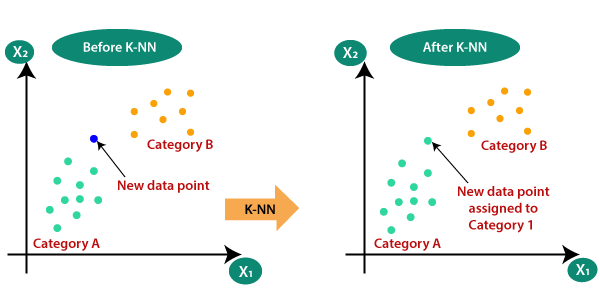
\includegraphics[width=1\linewidth]{img/Graphics/knn-arch.png}
        \caption{kNN Working\\Source : Javatpoint}
        \label{knn-arch}
    \end{figure}

    \begin{figure}[h]
        \centering
        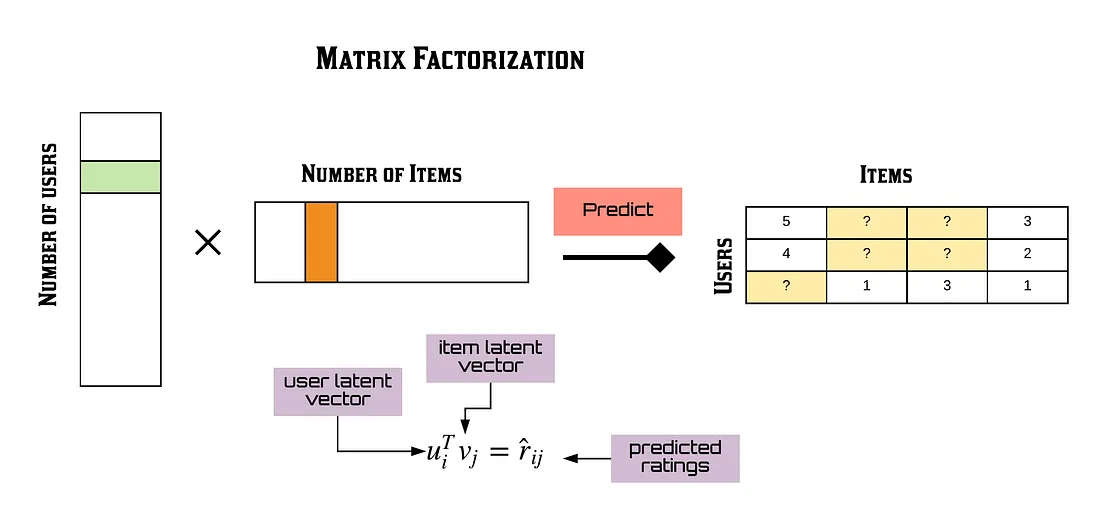
\includegraphics[width=1\linewidth]{img/Graphics/svd-arch.png}
        \caption{SVD Working\\Source : towardsdatascience}
        \label{svd-arch}
    \end{figure}
\newpage

    \begin{figure}[h]
        \centering
        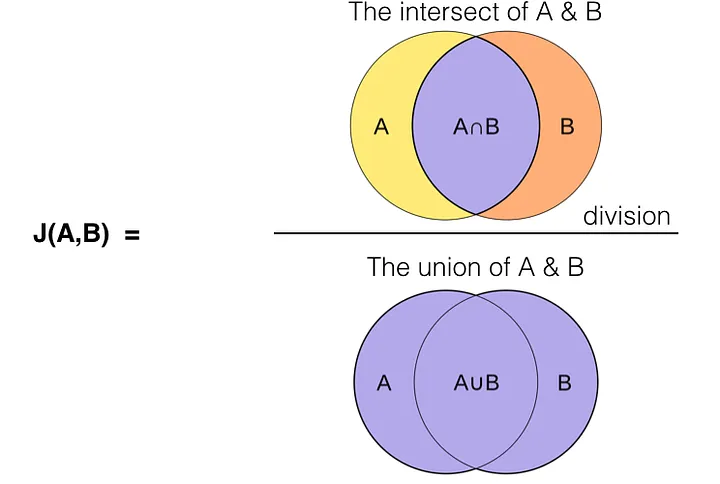
\includegraphics[width=0.8\linewidth]{img/Graphics/js-working.png}
        \caption{Jaccard's Similarity Working\\Source : medium.com/@aliozan\_memetoglu/}
        \label{js-working}
    \end{figure}
    
    \begin{figure}[h]
        \centering
        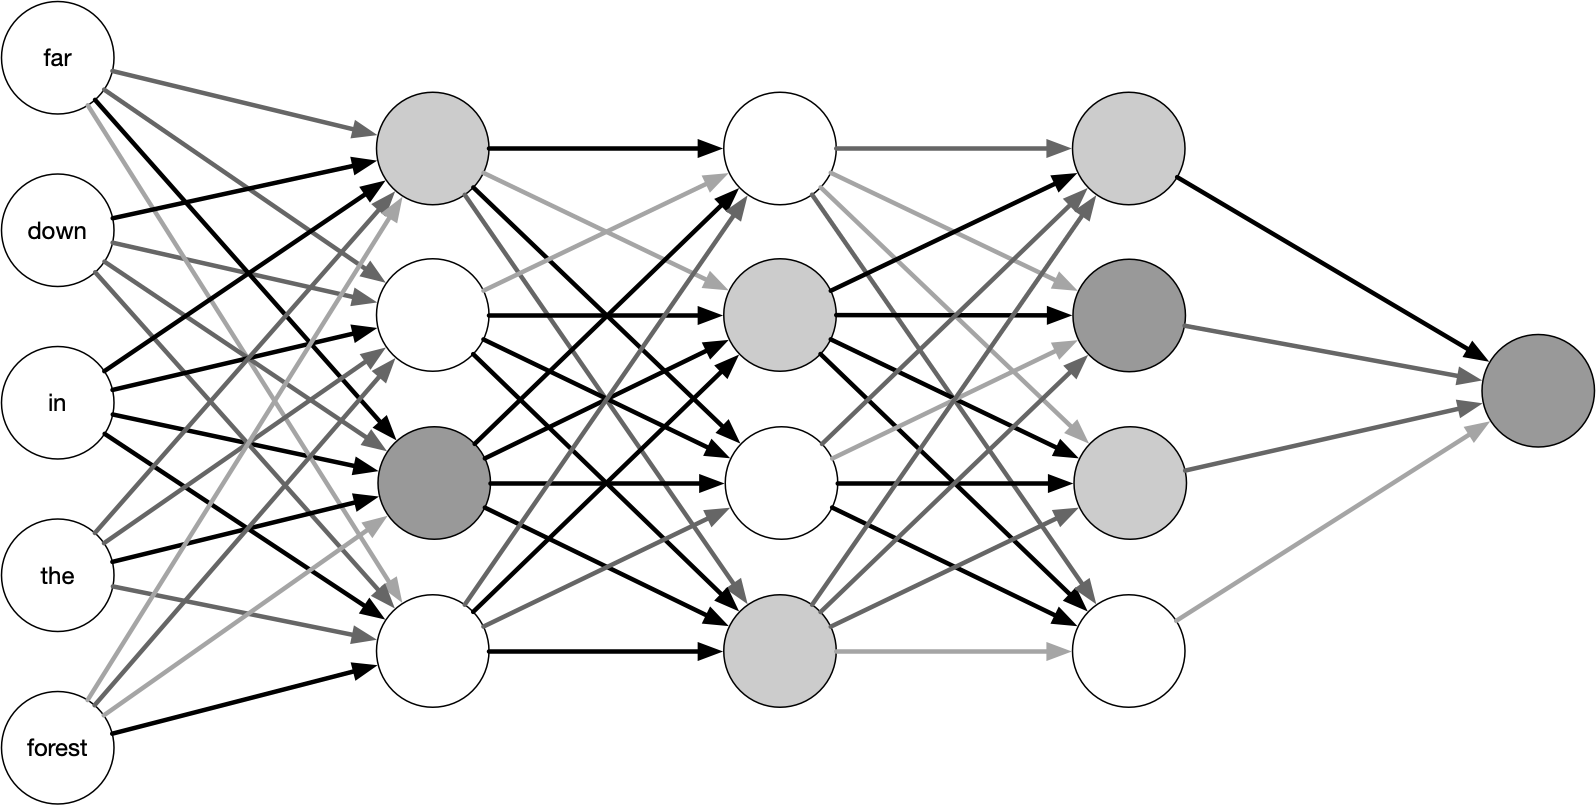
\includegraphics[width=1\linewidth]{img/Graphics/dense-nn.png}
        \caption{Dense Neural Network\\Source : \url{https://smltar.com/dldnn}}
        \label{dense-nn}
    \end{figure}
    \newpage
 \newpage

